Observa los camiones de la figura \ref{fig:camiones}, responde y argumenta.

\begin{minipage}[t]{0.7\linewidth}
    \begin{parts}
        \part ¿Cuál de ellos será más fácil poner en movimiento?
        \part ¿Cuál podría aumentar más rápido su velocidad?
        \part Si ambos se mueven a la misma velocidad, ¿a cuál le resultaría más difícil frenar?,
        ¿ambos podrían tomar una curva con la misma facilidad?
        \part Imagina que el camión cargado tira gradualmente parte de su cargamento,
        y que el conductor pisa el acelerador con la misma fuerza y mantiene el volante en la misma dirección.
        ¿Qué piensas que pasará con su rapidez?, ¿y si en vez de perder carga fuera recibiendo más?
    \end{parts}
\end{minipage}\hfill
\begin{minipage}[t]{0.25\linewidth}
    \begin{figure}[H]
        \centering
        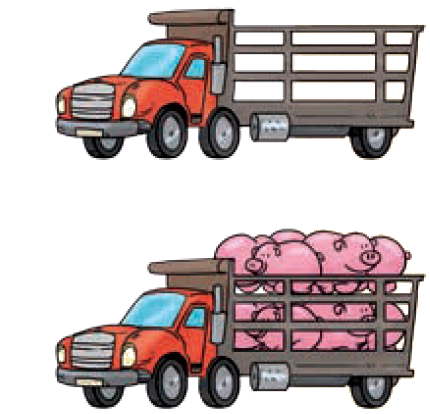
\includegraphics[width=\linewidth]{camiones.png}
        \captionof{figure}{Comparación de dos camiones con diferente masa.}
        \label{fig:camiones}
    \end{figure}
\end{minipage}